% Standalone Overleaf source. Compile with pdfLaTeX. No image files required.
\documentclass[10pt,a4paper]{article}
\usepackage[T1]{fontenc}
\usepackage[utf8]{inputenc}
\usepackage{lmodern,amsmath,amssymb,booktabs,tabularx,array,graphicx,float,microtype}
\usepackage[margin=0.8in]{geometry}
\usepackage{xcolor,hyperref,tikz,pgfplots,listings}
% Each pointer names a function and its location in the accompanying project.
\newcommand{\codeptr}[3]{\texttt{\detokenize{#2}()} (\path{#1}:#3)}
\lstdefinestyle{reportcode}{
  language=Python,basicstyle=\ttfamily\footnotesize,
  keywordstyle=\color{accent},commentstyle=\color{black!55},
  backgroundcolor=\color{black!3},rulecolor=\color{black!25},
  frame=single,framerule=.3pt,framesep=5pt,
  breaklines=true,breakatwhitespace=false,columns=fullflexible,
  keepspaces=true,showstringspaces=false,captionpos=b,
  aboveskip=.7em,belowskip=.7em
}
\pgfplotsset{compat=1.18,every axis/.append style={axis lines=left,tick label style={font=\small},label style={font=\small},scaled ticks=false}}
\definecolor{accent}{HTML}{244A63}
\hypersetup{colorlinks=true,urlcolor=accent,linkcolor=accent,pdftitle={Can Machine Learning Understand My Anime Taste?}}
\setlength{\parindent}{0pt}\setlength{\parskip}{0.65em}
\setlength{\emergencystretch}{3em}
\begin{document}

{\huge\bfseries\color{accent} Can Machine Learning Understand My Anime Taste?\par}\vspace{.5em}
{\small CS156 | Machine Learning Pipeline Assignment 1 | October 18, 2026\par}\vspace{1em}

\section*{1. What can my anime list predict?}
I can name genres and studios I usually enjoy, but that does not tell me which anime will become favorites. I used my MyAnimeList archive to test whether tags, studios, release year, episode count, and format contain enough information to predict my ratings. This is a supervised learning problem: the models learn from titles with known ratings, then make predictions for titles kept out of training. I compare predicting the score itself with identifying favorites, which I define as titles rated 10/10.

My rating scale matters to both tasks. A 10 means a favorite, a 9 means I liked it a lot, and a 7 or 8 means it did not affect me as strongly. The very low scores reflect anime I hated, so I kept them. Removing those scores as outliers would remove preferences I want the model to recognize. The scale is ordered, but a change from 9 to 10 may mean something different to me than a change from 1 to 2. Regression approximates these judgments as equally spaced numbers. The favorite task uses 10 as a clear class boundary in my scale.

\subsection*{The ratings}
The export contains 357 distinct titles: 306 rated and 51 unrated. Of the rated titles, 235 (76.8\%) have scores of 8-10. I used the 294 completed, rated titles for the main experiment because ratings for unfinished shows reflect different amounts of viewing. I retained the other 12 rated entries for a development-only sensitivity check. A score of 0 means unrated and is excluded from the labels.
\begin{figure}[H]\centering
\begin{minipage}[t]{1\linewidth}\centering
\resizebox{\linewidth}{!}{%
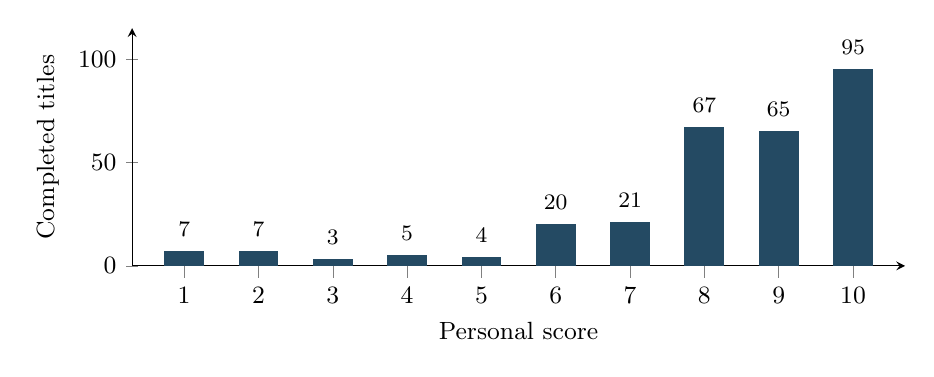
\begin{tikzpicture}\begin{axis}[clip=false,axis lines=left,scaled ticks=false,tick label style={font=\small},label style={font=\small},title style={font=\small},legend cell align=left,legend style={font=\scriptsize,draw=none,fill=white,at={(.5,.98)},anchor=north},width=.94\linewidth,height=4.6cm,ybar,bar width=14pt,xmin=.3,xmax=10.7,ymin=0,ymax=115,xtick={1,...,10},xlabel={Personal score},ylabel={Completed titles},nodes near coords,every node near coord/.append style={font=\footnotesize,yshift=2pt}]
\addplot[fill=accent,draw=accent] coordinates {(1.00000,7.00000) (2.00000,7.00000) (3.00000,3.00000) (4.00000,5.00000) (5.00000,4.00000) (6.00000,20.00000) (7.00000,21.00000) (8.00000,67.00000) (9.00000,65.00000) (10.00000,95.00000)};
\end{axis}\end{tikzpicture}%
}
\end{minipage}\par\vspace{.3em}{\footnotesize Figure 1. Completed, rated titles (n=294): mean 8.19, median 9, and 95 favorites rated 10.}\end{figure}
Figure 1 shows why a baseline is necessary. A model could make fairly small errors by predicting a high score for everything, without learning much about my preferences. I therefore compare every learned regressor with predictions based only on the training mean or median. I also examine lower scores separately, using a 1-6 band without assuming that every title in that band is one I hated.

\clearpage

\section*{2. Preparing the data and separating the tests}
The parser reads plain or gzipped XML, converts IDs, scores, and episode counts to integers, and checks score bounds and duplicate IDs. The shared copy keeps the six fields used here and omits account information. All 357 entries matched metadata by exact MyAnimeList ID. The parser is \codeptr{src/ingest.py}{parse_export}{21}.\footnote{Code pointers give a function, a project-relative file path, and a source line in this version of the project.}

Jikan requests timed out, so I used Anime Offline Database release 2026-27 and saved the matching records locally. Its July 4, 2026 snapshot predates my October export. The project records its source, dates, file hashes, and license, allowing the notebook to run without a live API [1-3].
\begin{figure}[H]\centering
\resizebox{\linewidth}{!}{%
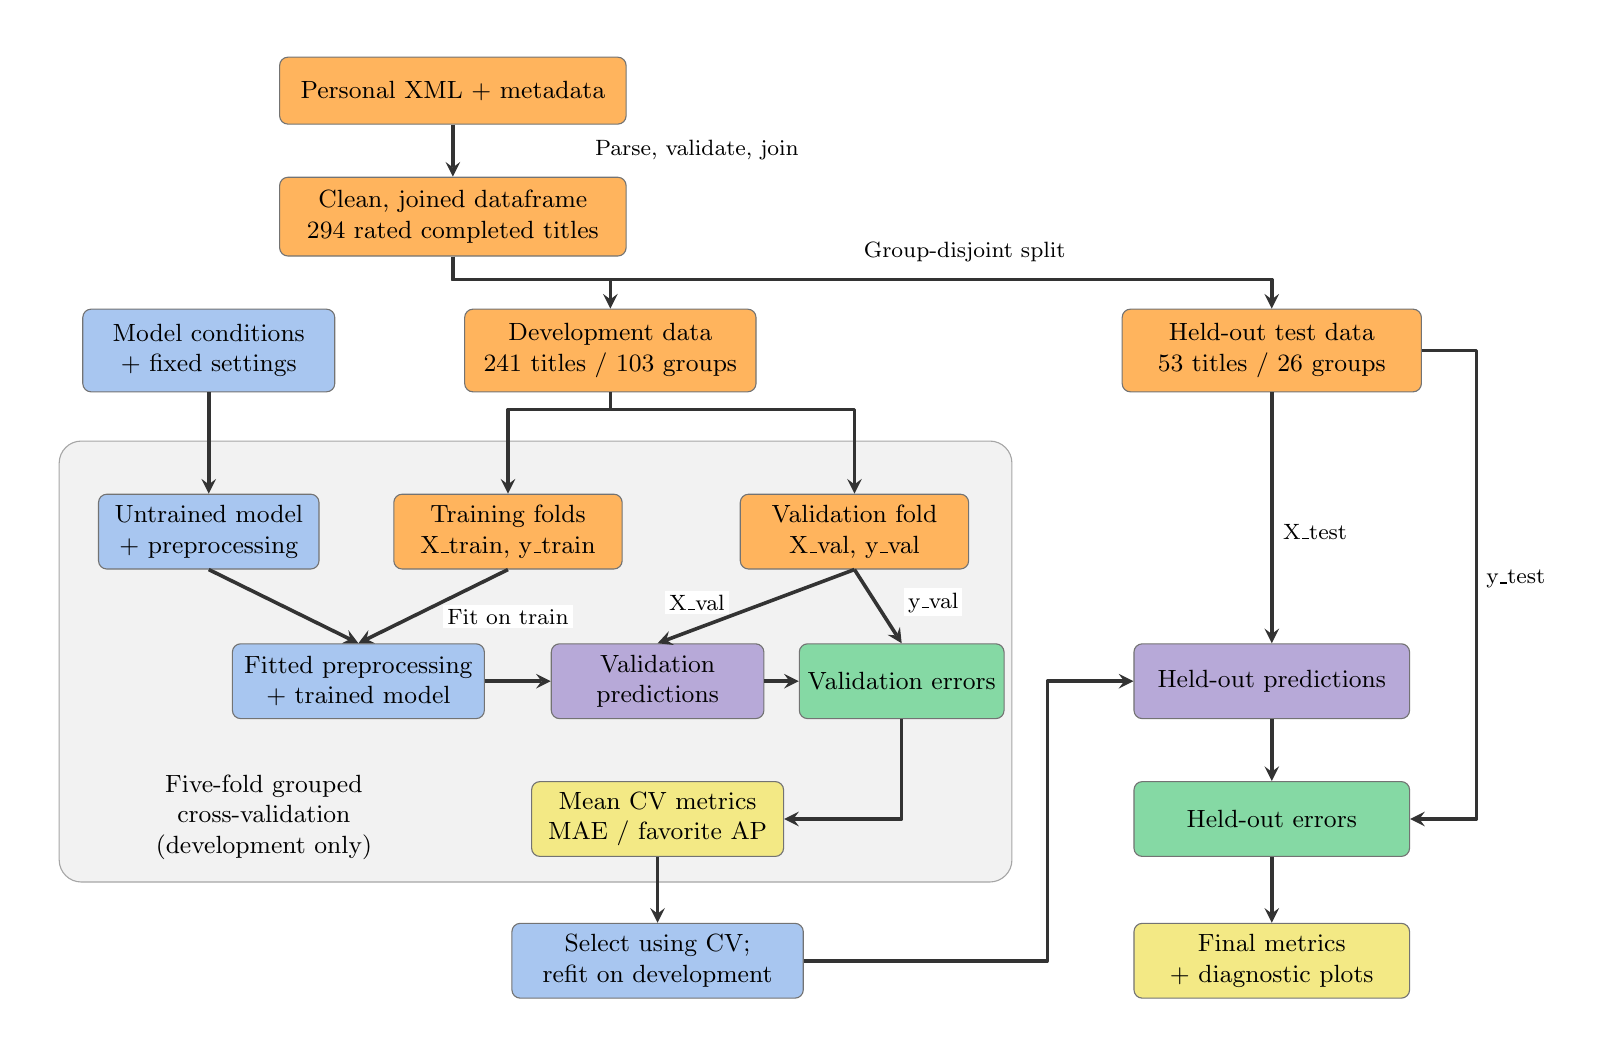
\begin{tikzpicture}[>=stealth,line join=round,
box/.style={draw=black!55,rounded corners=3pt,align=center,font=\small,inner sep=3pt},
flow/.style={->,draw=black!80,line width=1.3pt},
edge label/.style={font=\footnotesize,fill=white,inner sep=1.5pt,align=center}]
\path[use as bounding box] (-.4,-1.1) rectangle (19.2,11.5);
\filldraw[fill=black!5,draw=black!35,rounded corners=8pt] (0,.65) rectangle (12.1,6.25);
\node[align=center,font=\small] at (2.6,1.47) {Five-fold grouped\\cross-validation\\(development only)};
\definecolor{noderaw}{HTML}{FFB45D}
\node[box,fill=noderaw,minimum width=4.4cm,minimum height=0.85cm] (raw) at (5,10.7) {Personal XML + metadata};
\definecolor{nodeframe}{HTML}{FFB45D}
\node[box,fill=nodeframe,minimum width=4.4cm,minimum height=1.0cm] (frame) at (5,9.1) {Clean, joined dataframe\\294 rated completed titles};
\definecolor{nodechoices}{HTML}{A8C6F0}
\node[box,fill=nodechoices,minimum width=3.2cm,minimum height=1.05cm] (choices) at (1.9,7.4) {Model conditions\\+ fixed settings};
\definecolor{nodedev}{HTML}{FFB45D}
\node[box,fill=nodedev,minimum width=3.7cm,minimum height=1.05cm] (dev) at (7,7.4) {Development data\\241 titles / 103 groups};
\definecolor{nodetest}{HTML}{FFB45D}
\node[box,fill=nodetest,minimum width=3.8cm,minimum height=1.05cm] (test) at (15.4,7.4) {Held-out test data\\53 titles / 26 groups};
\definecolor{nodemodel}{HTML}{A8C6F0}
\node[box,fill=nodemodel,minimum width=2.8cm,minimum height=0.95cm] (model) at (1.9,5.1) {Untrained model\\+ preprocessing};
\definecolor{nodetrain}{HTML}{FFB45D}
\node[box,fill=nodetrain,minimum width=2.9cm,minimum height=0.95cm] (train) at (5.7,5.1) {Training folds\\X\_train, y\_train};
\definecolor{nodeval}{HTML}{FFB45D}
\node[box,fill=nodeval,minimum width=2.9cm,minimum height=0.95cm] (val) at (10.1,5.1) {Validation fold\\X\_val, y\_val};
\definecolor{nodefit}{HTML}{A8C6F0}
\node[box,fill=nodefit,minimum width=3.2cm,minimum height=0.95cm] (fit) at (3.8,3.2) {Fitted preprocessing\\+ trained model};
\definecolor{nodepred}{HTML}{B7A9D8}
\node[box,fill=nodepred,minimum width=2.7cm,minimum height=0.95cm] (pred) at (7.6,3.2) {Validation\\predictions};
\definecolor{nodeerr}{HTML}{85D9A4}
\node[box,fill=nodeerr,minimum width=2.6cm,minimum height=0.95cm] (err) at (10.7,3.2) {Validation errors};
\definecolor{nodecvmetrics}{HTML}{F3E985}
\node[box,fill=nodecvmetrics,minimum width=3.2cm,minimum height=0.95cm] (cvmetrics) at (7.6,1.45) {Mean CV metrics\\MAE / favorite AP};
\definecolor{nodeselected}{HTML}{A8C6F0}
\node[box,fill=nodeselected,minimum width=3.7cm,minimum height=0.95cm] (selected) at (7.6,-0.35) {Select using CV;\\refit on development};
\definecolor{nodetestpred}{HTML}{B7A9D8}
\node[box,fill=nodetestpred,minimum width=3.5cm,minimum height=0.95cm] (testpred) at (15.4,3.2) {Held-out predictions};
\definecolor{nodetesterr}{HTML}{85D9A4}
\node[box,fill=nodetesterr,minimum width=3.5cm,minimum height=0.95cm] (testerr) at (15.4,1.45) {Held-out errors};
\definecolor{nodefinal}{HTML}{F3E985}
\node[box,fill=nodefinal,minimum width=3.5cm,minimum height=0.95cm] (final) at (15.4,-0.35) {Final metrics\\+ diagnostic plots};
\draw[flow] (raw.south) -- (frame.north);
\node[edge label] at (8.1,9.95) {Parse, validate, join};
\draw[flow] (frame.south) -- (5,8.3) -- (7,8.3) -- (dev.north);
\draw[flow] (frame.south) -- (5,8.3) -- (15.4,8.3) -- (test.north);
\node[edge label] at (11.5,8.65) {Group-disjoint split};
\draw[flow] (choices.south) -- (model.north);
\draw[flow] (dev.south) -- (7,6.65) -- (5.7,6.65) -- (train.north);
\draw[flow] (dev.south) -- (7,6.65) -- (10.1,6.65) -- (val.north);
\draw[flow] (model.south) -- (fit.north);
\draw[flow] (train.south) -- (fit.north);
\node[edge label] at (5.7,4.02) {Fit on train};
\draw[flow] (fit.east) -- (pred.west);
\draw[flow] (val.south) -- (pred.north);
\node[edge label] at (8.1,4.2) {X\_val};
\draw[flow] (val.south) -- (err.north);
\node[edge label] at (11.1,4.2) {y\_val};
\draw[flow] (pred.east) -- (err.west);
\draw[flow] (err.south) -- (10.7,1.45) -- (cvmetrics.east);
\draw[flow] (cvmetrics.south) -- (selected.north);
\draw[flow] (selected.east) -- (12.55,-0.35) -- (12.55,3.2) -- (testpred.west);
\draw[flow] (test.south) -- (testpred.north);
\node[edge label] at (15.95,5.1) {X\_test};
\draw[flow] (test.east) -- (18,7.4) -- (18,1.45) -- (testerr.east);
\node[edge label] at (18.5,4.5) {y\_test};
\draw[flow] (testpred.south) -- (testerr.north);
\draw[flow] (testerr.south) -- (final.north);\end{tikzpicture}}\par\vspace{.3em}{\footnotesize Figure 2. Cross-validation uses development groups only. Each fold fits its own preprocessing and model; test groups enter the final evaluation after model selection.}\end{figure}
In Figure 2, \(X\) contains anime features and \(y\) contains my ratings. I selected 43 broad genre and theme tags from the source's aggregated taxonomy. Tags and studios use multi-hot encoding: Action and Drama activate separate binary columns. Format uses one-hot encoding, with columns for categories such as TV and movie. These encodings avoid assigning a numerical order to categories. The transformations are assembled in \codeptr{src/pipeline.py}{preprocessing}{77}.

The numeric features are release year and \(\log(1+E)\), where \(E\) is episode count from the export. The logarithm compresses differences between short and long series. Standardization based on training rows puts these inputs on comparable scales for the penalized models and network. Median imputation handles missing values, although none occur in the main sample. The full development fit creates 147 features. I exclude titles and IDs to discourage memorization, watch status and progress because they describe my viewing behavior, and community ratings to focus the question on descriptive metadata. Feature preparation is implemented in \codeptr{src/pipeline.py}{load_data}{52}.

To reduce leakage between related titles, I built a graph from links across all 41,537 metadata records, including titles outside my list. Titles connected directly or through other titles stay together, forming 129 groups in the main sample. With seed 42, 103 groups (241 titles) enter development and 26 groups (53 titles) enter the held-out test set. Keeping seasons together tests transfer to unseen relation groups [4-5]. The graph construction and component assignment are in \codeptr{src/ingest.py}{make_snapshot}{62}.

Five-fold grouped cross-validation trains on four development folds and validates on the fifth, rotating through all five. Each training fold learns its encoding vocabulary, imputation values, and scaling statistics; validation data use those fitted transformations. After selection, each model is refitted on all development data and evaluated on the same test set. Test labels do not choose the model or its settings. The fold loop is \codeptr{src/pipeline.py}{fit_cv}{172}, which creates a fresh preprocessing/model pipeline through \codeptr{src/pipeline.py}{make_pipe}{162}.

Crossovers and adaptations make these groups broader than verified franchises. The largest contains 87 completed titles, producing uneven validation folds of 119, 32, 30, 32, and 28 titles. I give each fold equal weight in the mean validation error. Fold standard deviation describes their variation; it is not a confidence interval.

\clearpage

\section*{3. How the models learn}
\begin{center}\small\renewcommand{\arraystretch}{1.35}\begin{tabularx}{\textwidth}{@{}lX@{}}\toprule
\textbf{Condition} & \textbf{Fixed training settings}\\\midrule
Mean / median & Training-label constant; no explanatory features\\
Ridge & L2 penalty \(\alpha=10\); additive linear effects\\
Decision tree & Maximum depth 4; minimum 8 samples per leaf\\
Neural network & 16 and 8 ReLU units; L2=10; L-BFGS; standardized target\\
Favorite classifier & Class-weighted logistic; \(C=0.1\); threshold 0.5\\
\bottomrule\end{tabularx}\end{center}
The regression configurations in this table are defined in \codeptr{src/pipeline.py}{regressors}{110}.

\textbf{Baselines.} The mean and median baselines each predict one constant calculated from training ratings. The mean minimizes training squared error among constant predictions; the median minimizes training absolute error. Because my scores are concentrated near the top, these are meaningful competitors.

\textbf{Ridge regression.} Ridge predicts a weighted sum of features. For a binary tag, its coefficient describes how much that tag changes the unbounded prediction when the other encoded inputs are held fixed:
\[
\begin{aligned}
\hat y_i &= b+x_i^\top\beta,\\
(\hat b,\hat\beta) &= \arg\min_{b,\beta}
\left[\sum_{i=1}^{n}(y_i-b-x_i^\top\beta)^2+10\|\beta\|_2^2\right].
\end{aligned}
\]
Here, \(x_i\) is the feature vector, \(y_i\) is my rating, \(b\) is the intercept, and \(\beta\) contains the feature weights. The first term rewards fitting the training ratings. The second penalizes large weights, reducing reliance on rare or correlated features. I fixed its strength at 10 because 147 encoded features are many relative to 241 development titles, making an unrestricted fit vulnerable to overfitting [6]. Ridge still assumes additive effects, so a tag contributes the same amount across different combinations of other features.

\textbf{Decision tree.} A tree repeatedly splits training titles at feature thresholds to reduce squared error. Each leaf predicts the mean training rating of the titles reaching it. Because later splits depend on earlier ones, the tree can learn interactions---for example, that a tag predicts different ratings for TV series and movies. Maximum depth 4 and at least 8 samples per leaf limit the small, specific groups it can memorize [8].

\textbf{Neural network.} The network passes features through hidden layers of 16 and 8 units, then a linear output. Each hidden unit applies ReLU, \(r(a)=\max(0,a)\), to a weighted sum of its inputs. These nonlinear transformations let the model learn combinations of features beyond ridge's additive effects. L-BFGS uses loss gradients to adjust the weights, minimizing squared error with an L2 penalty of 10 over at most 3,000 iterations. The target is standardized using training labels, then predictions are converted back to rating points [9].

All score predictions are clipped to [1,10] without rounding. I compared these fixed configurations without a hyperparameter search; settings were fixed before test evaluation.

\subsection*{Choosing a regressor}
The learned regressors fit squared-error objectives, but I select between them using mean absolute error (MAE), because an average miss in rating points is easy to interpret:
\[
\mathrm{MAE}=\frac{1}{n}\sum_{i=1}^{n}|y_i-\hat y_i|,
\qquad
\mathrm{RMSE}=\sqrt{\frac{1}{n}\sum_{i=1}^{n}(y_i-\hat y_i)^2}.
\]
For evaluation, \(n\) is the number of evaluated titles and \(\hat y_i\) is the final prediction. Predicting 8 for a rating of 9 contributes one point to absolute error. Root mean squared error (RMSE) gives large misses more influence. I also report the share within one point and error by rating band. Macro-score MAE averages the MAE for each exact score present in the test set, giving rare and common scores equal weight. These measures reveal errors that an overall average can hide. Their implementation is \codeptr{src/pipeline.py}{score_regression}{133}.

\subsection*{Identifying favorites}
For the second task, a title is positive only when its rating is 10:
\[
z_i=\mathbf{1}[y_i=10],\qquad
p_i=\frac{1}{1+\exp[-(b_c+w^\top x_i)]}.
\]
Logistic regression learns weights \(w\) and intercept \(b_c\), producing an output \(p_i\) between 0 and 1. It minimizes weighted log loss, which penalizes confident wrong predictions, with L2 regularization. I used \(C=0.1\); smaller \(C\) means stronger regularization. Inverse-frequency class weights give both classes equal total training weight. The baseline assigns every title the training favorite share. Because weighting changes the fitted objective, I use logistic outputs for ranking without assuming they are calibrated personal probabilities [10].

The classification loop in \codeptr{src/pipeline.py}{run_experiments}{296} applies the definition of a favorite directly to the training labels. The following lines fit the full pipeline on training rows and extract class-1 outputs for validation rows.
\begin{lstlisting}[style=reportcode,caption={Favorite target and validation predictions, src/pipeline.py:296--297.}]
pipe = make_pipe(model).fit(Xd.iloc[tr], (yd.iloc[tr] == 10).astype(int))
prob = pipe.predict_proba(Xd.iloc[va])[:, 1]
\end{lstlisting}

I select the classifier using mean validation average precision (AP):
\[
\mathrm{AP}=\sum_k(R_k-R_{k-1})P_k.
\]
Starting with the highest-ranked titles, precision \(P_k\) is the fraction selected that are favorites, and recall \(R_k\) is the fraction of all favorites recovered. AP weights precision by each increase in recall as the threshold is lowered, matching the goal of finding favorites near the top of a list [7]. ROC AUC checks how often favorites rank above nonfavorites. Balanced accuracy averages recall for both classes at a fixed 0.5 threshold, while Brier score measures mean squared probability error. Higher AP, ROC AUC, and balanced accuracy are better; lower Brier score is better [11].

\clearpage

\section*{4. How the models performed}
\begin{center}\small\renewcommand{\arraystretch}{1.35}\begin{tabularx}{\textwidth}{@{}Xrrrr@{}}\toprule
\textbf{Model} & \textbf{CV MAE (SD)} & \textbf{Test MAE} & \textbf{Test RMSE} & \textbf{Macro MAE}\\\midrule
Mean baseline & 1.575 (0.362) & 1.431 & 2.004 & 2.346\\
Median baseline & 1.489 (0.360) & 1.415 & 2.070 & 2.714\\
Ridge regression & 1.421 (0.378) & 1.446 & 1.828 & 1.907\\
Decision tree & 1.770 (0.316) & 1.514 & 2.183 & 1.950\\
Neural network & 1.455 (0.284) & 1.506 & 1.825 & 1.659\\
\bottomrule\end{tabularx}\end{center}
Ridge had the lowest mean validation MAE: 1.421, compared with 1.489 for the median baseline. That made ridge the selected regressor before test evaluation. On the 53 test titles, its MAE was 1.446 versus 1.415 for predicting the training median of 9. None of the learned regressors beat that baseline on test MAE. The validation-based choice and subsequent test fits are in \codeptr{src/pipeline.py}{run_experiments}{269}.

The observed difference between ridge and the median baseline was only 0.031 points in the baseline's favor. To check its sensitivity to the test groups, I resampled the 26 groups with replacement 2,000 times, keeping related titles together. The 95\% bootstrap interval for ridge MAE minus baseline MAE was [-0.595, 0.369]. Because it includes improvements and losses, it provides no clear evidence of an overall MAE advantage. It describes variation in the fixed test comparison, without accounting for retraining or choosing another split.

The bootstrap loop below is in \codeptr{src/pipeline.py}{run_experiments}{325}. Here, \texttt{diffs} stores each title's learned-model absolute error minus its baseline absolute error. Each draw selects complete test groups, and \texttt{ix} gathers all their row positions before averaging the paired differences.
\begin{lstlisting}[style=reportcode,caption={Paired group bootstrap, src/pipeline.py:325--331; comments omitted.}]
for _ in range(2000):
    chosen = rng.choice(unique, size=len(unique), replace=True)
    ix = np.concatenate([np.flatnonzero(gt.to_numpy() == g) for g in chosen])
    draws.append(diffs[ix].mean())
\end{lstlisting}

\begin{figure}[H]\centering
\begin{minipage}[t]{.57\linewidth}\centering
\resizebox{\linewidth}{!}{%
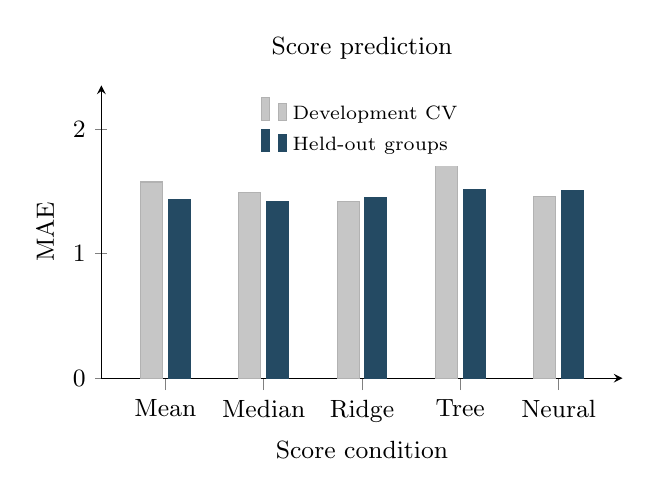
\begin{tikzpicture}\begin{axis}[clip=false,axis lines=left,scaled ticks=false,tick label style={font=\small},label style={font=\small},title style={font=\small},legend cell align=left,legend style={font=\scriptsize,draw=none,fill=white,at={(.5,.98)},anchor=north},width=8.2cm,height=5.3cm,ybar,bar width=8pt,xmin=.35,xmax=5.65,ymin=0,ymax=2.35,xtick={1,2,3,4,5},xticklabels={Mean,Median,Ridge,Tree,Neural},xlabel={Score condition},ylabel={MAE},title={Score prediction}]
\addplot[fill=gray!45,draw=gray!60] coordinates {(1.00000,1.57482) (2.00000,1.48865) (3.00000,1.42059) (4.00000,1.76978) (5.00000,1.45545)};
\addplot[fill=accent,draw=accent] coordinates {(1.00000,1.43130) (2.00000,1.41509) (3.00000,1.44606) (4.00000,1.51450) (5.00000,1.50608)};
\legend{Development CV,Held-out groups}\end{axis}\end{tikzpicture}%
}
\end{minipage}
\hfill
\begin{minipage}[t]{.40\linewidth}\centering
\resizebox{\linewidth}{!}{%
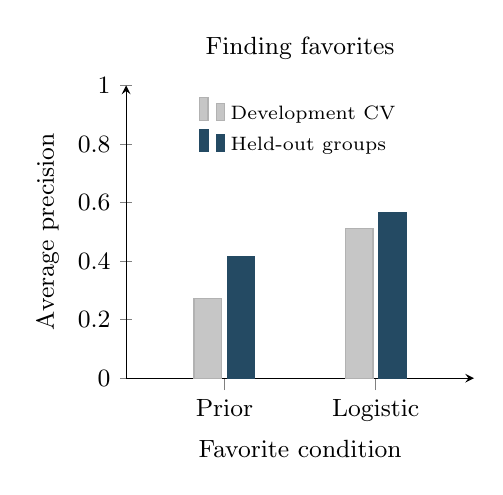
\begin{tikzpicture}\begin{axis}[clip=false,axis lines=left,scaled ticks=false,tick label style={font=\small},label style={font=\small},title style={font=\small},legend cell align=left,legend style={font=\scriptsize,draw=none,fill=white,at={(.5,.98)},anchor=north},width=6cm,height=5.3cm,ybar,bar width=10pt,xmin=.35,xmax=2.65,ymin=0,ymax=1,xtick={1,2},xticklabels={Prior,Logistic},xlabel={Favorite condition},ylabel={Average precision},title={Finding favorites}]
\addplot[fill=gray!45,draw=gray!60] coordinates {(1.00000,0.27356) (2.00000,0.51273)};
\addplot[fill=accent,draw=accent] coordinates {(1.00000,0.41509) (2.00000,0.56541)};
\legend{Development CV,Held-out groups}\end{axis}\end{tikzpicture}%
}
\end{minipage}\par\vspace{.3em}{\footnotesize Figure 3. Score prediction and favorite classification. Lower MAE and higher AP are better; development and test results use different title groups.}\end{figure}\begin{center}\small\renewcommand{\arraystretch}{1.35}\begin{tabularx}{\textwidth}{@{}Xrrrr@{}}\toprule
\textbf{Favorite condition} & \textbf{CV AP (SD)} & \textbf{Test AP} & \textbf{ROC AUC} & \textbf{Bal. acc.}\\\midrule
Prior baseline & 0.274 (0.067) & 0.415 & 0.500 & 0.500\\
Favorite logistic & 0.513 (0.249) & 0.565 & 0.570 & 0.559\\
\bottomrule\end{tabularx}\end{center}
For favorites, logistic regression increased mean validation AP from 0.274 to 0.513, although fold results varied substantially (SD 0.249). Test AP was 0.565 versus 0.415. AP is a ranking measure; 0.565 does not mean that 56.5\% of titles were classified correctly. The constant baseline ranks all titles equally, so its AP equals the evaluated favorite share: 22/53 on the test set. Because that share changes between folds and test data, the baseline must be compared within the same evaluation population.

The other metrics limit how strongly I interpret this improvement. Test ROC AUC was 0.570 and balanced accuracy was 0.559, both close to their 0.5 baselines. Brier score fell slightly, from 0.255 to 0.251. The model shows some ranking information on this test set, but it does not separate favorites from other titles reliably enough to claim strong performance.

The tree's score predictions produced test favorite AP of 0.600. Switching to it after seeing that result would reuse the test set for selection, so I kept the models chosen using development data.

\clearpage

\section*{5. Where predictions miss my preferences}
\begin{figure}[H]\centering
\begin{minipage}[t]{.48\linewidth}\centering
\resizebox{\linewidth}{!}{%
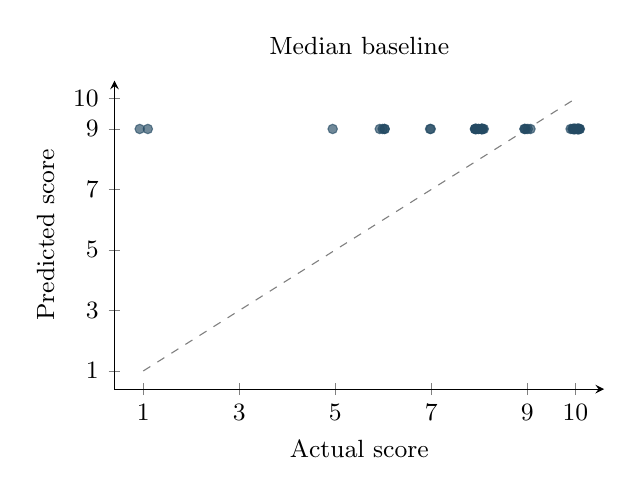
\begin{tikzpicture}\begin{axis}[clip=false,axis lines=left,scaled ticks=false,tick label style={font=\small},label style={font=\small},title style={font=\small},legend cell align=left,legend style={font=\scriptsize,draw=none,fill=white,at={(.5,.98)},anchor=north},width=7.8cm,height=5.5cm,xmin=.4,xmax=10.6,ymin=.4,ymax=10.6,xtick={1,3,5,7,9,10},ytick={1,3,5,7,9,10},xlabel={Actual score},ylabel={Predicted score},title={Median baseline}]
\addplot[no marks,dashed,color=gray] coordinates {(1,1) (10,10)};
\addplot[only marks,mark=*,mark size=1.7pt,color=accent,opacity=.65] coordinates {(8.05479,9.00000) (9.98778,9.00000) (8.07172,9.00000) (8.03947,9.00000) (7.91884,9.00000) (1.09512,9.00000) (10.05223,9.00000) (8.05721,9.00000) (0.92562,9.00000) (7.99008,9.00000) (6.97416,9.00000) (10.08535,9.00000) (6.02877,9.00000) (8.06455,9.00000) (6.98868,9.00000) (4.94545,9.00000) (9.01092,9.00000) (7.91276,9.00000) (10.06553,9.00000) (6.02633,9.00000) (8.05162,9.00000) (8.97091,9.00000) (10.09414,9.00000) (10.07862,9.00000) (10.05568,9.00000) (9.93893,9.00000) (9.99334,9.00000) (7.90876,9.00000) (7.93086,9.00000) (8.03661,9.00000) (8.04895,9.00000) (8.09350,9.00000) (9.96517,9.00000) (7.97409,9.00000) (9.99391,9.00000) (7.93789,9.00000) (5.92598,9.00000) (9.99514,9.00000) (8.94538,9.00000) (10.03396,9.00000) (5.98743,9.00000) (9.06654,9.00000) (10.04005,9.00000) (9.96247,9.00000) (10.06645,9.00000) (10.06095,9.00000) (9.97750,9.00000) (9.95767,9.00000) (10.03650,9.00000) (7.92795,9.00000) (8.93998,9.00000) (9.90147,9.00000) (10.05738,9.00000)};
\end{axis}\end{tikzpicture}%
}
\end{minipage}
\hfill
\begin{minipage}[t]{.48\linewidth}\centering
\resizebox{\linewidth}{!}{%
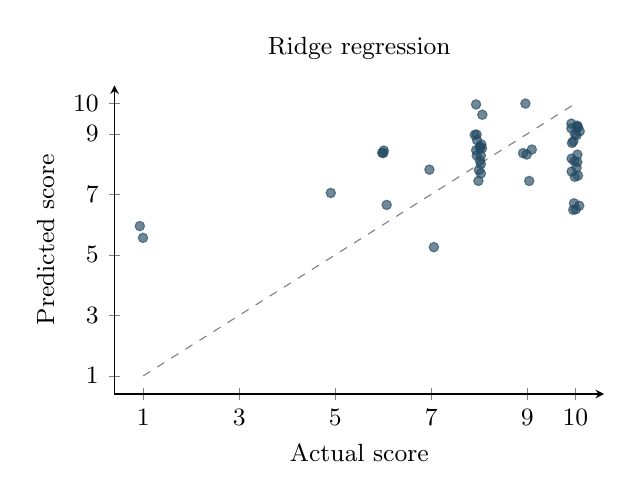
\begin{tikzpicture}\begin{axis}[clip=false,axis lines=left,scaled ticks=false,tick label style={font=\small},label style={font=\small},title style={font=\small},legend cell align=left,legend style={font=\scriptsize,draw=none,fill=white,at={(.5,.98)},anchor=north},width=7.8cm,height=5.5cm,xmin=.4,xmax=10.6,ymin=.4,ymax=10.6,xtick={1,3,5,7,9,10},ytick={1,3,5,7,9,10},xlabel={Actual score},ylabel={Predicted score},title={Ridge regression}]
\addplot[no marks,dashed,color=gray] coordinates {(1,1) (10,10)};
\addplot[only marks,mark=*,mark size=1.7pt,color=accent,opacity=.65] coordinates {(8.03297,7.69052) (10.04103,8.06582) (8.05615,8.52314) (7.99178,7.80199) (8.01375,8.53200) (0.92796,5.94937) (9.92291,8.18074) (8.03368,8.00096) (0.99422,5.56092) (8.01305,8.10974) (7.05300,5.25316) (10.02694,7.87803) (6.01072,8.44700) (8.01184,8.57834) (6.96079,7.81542) (4.90616,7.04476) (8.98734,8.31530) (7.94292,8.97664) (9.98171,8.09880) (6.07068,6.65053) (7.94679,8.28399) (8.91166,8.36224) (9.95628,6.48642) (9.95872,8.75118) (10.03238,9.22836) (10.01141,6.50371) (10.05678,7.61861) (8.03286,8.27925) (7.98128,7.44408) (8.06280,9.63180) (7.93339,8.45871) (7.90454,8.96495) (9.91801,9.33723) (8.04447,8.64762) (9.99238,8.99613) (7.93225,9.97046) (6.00021,8.36487) (9.93046,8.69848) (9.03926,7.44151) (9.98923,7.57826) (5.97620,8.37151) (8.96030,10.00000) (10.02606,8.95312) (9.97236,6.70293) (9.91753,9.18073) (9.92360,7.75396) (10.09238,9.08225) (10.08172,6.62290) (10.03994,9.26821) (7.95317,8.78850) (9.09384,8.48018) (10.05575,9.22145) (10.04338,8.31310)};
\end{axis}\end{tikzpicture}%
}
\end{minipage}\par\vspace{.3em}{\footnotesize Figure 4. Predictions for 53 test titles. Horizontal jitter separates overlapping ratings; the dashed line marks perfect prediction.}\end{figure}
Figure 4 shows the median baseline's limitation: every prediction lies at 9, including predictions for titles I strongly disliked. It put 83.0\% of test titles within one point of my rating, but its MAE was 4.571 on the seven titles rated 1-6. Ridge was within one point less often (50.9\%), while reducing lower-band MAE to 2.770. Ridge also reduced RMSE from 2.070 to 1.828 and macro-score MAE from 2.714 to 1.907. It made smaller errors on low scores while undershooting many favorites. This explains how the median could win overall MAE despite making larger mistakes on the lower-rated titles. With only seven lower-band examples, that part of the comparison remains uncertain.
\begin{figure}[H]\centering
\begin{minipage}[t]{.48\linewidth}\centering
\resizebox{\linewidth}{!}{%
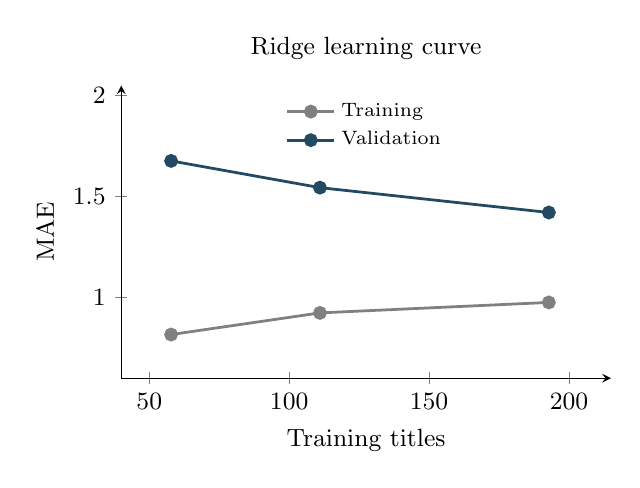
\begin{tikzpicture}\begin{axis}[clip=false,axis lines=left,scaled ticks=false,tick label style={font=\small},label style={font=\small},title style={font=\small},legend cell align=left,legend style={font=\scriptsize,draw=none,fill=white,at={(.5,.98)},anchor=north},width=7.8cm,height=5.3cm,xmin=40,xmax=215,ymin=.6,ymax=2.05,xlabel={Training titles},ylabel={MAE},title={Ridge learning curve}]
\addplot[color=gray,mark=*,line width=1pt] coordinates {(57.80000,0.81620) (111.00000,0.92341) (192.80000,0.97528)};
\addplot[color=accent,mark=*,line width=1pt] coordinates {(57.80000,1.67613) (111.00000,1.54371) (192.80000,1.42059)};
\legend{Training,Validation}\end{axis}\end{tikzpicture}%
}
\end{minipage}
\hfill
\begin{minipage}[t]{.48\linewidth}\centering
\resizebox{\linewidth}{!}{%
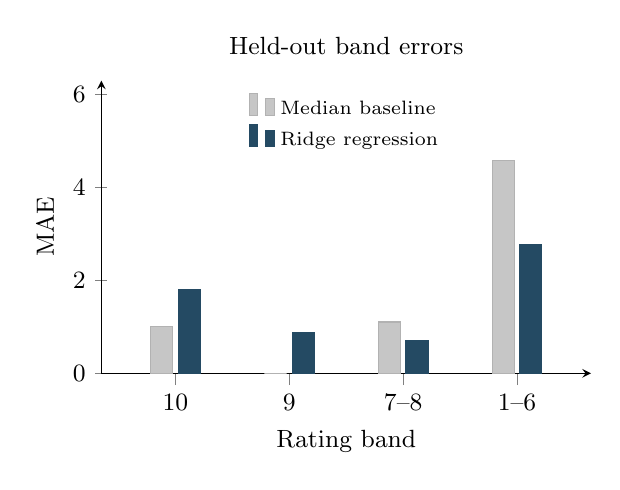
\begin{tikzpicture}\begin{axis}[clip=false,axis lines=left,scaled ticks=false,tick label style={font=\small},label style={font=\small},title style={font=\small},legend cell align=left,legend style={font=\scriptsize,draw=none,fill=white,at={(.5,.98)},anchor=north},width=7.8cm,height=5.3cm,ybar,bar width=8pt,xmin=.35,xmax=4.65,ymin=0,ymax=6.3,xtick={1,2,3,4},xticklabels={10,9,7--8,1--6},xlabel={Rating band},ylabel={MAE},title={Held-out band errors}]
\addplot[fill=gray!45,draw=gray!60] coordinates {(1.00000,1.00000) (2.00000,0.00000) (3.00000,1.10526) (4.00000,4.57143)};
\addplot[fill=accent,draw=accent] coordinates {(1.00000,1.79453) (2.00000,0.88016) (3.00000,0.70378) (4.00000,2.76985)};
\legend{Median baseline,Ridge regression}\end{axis}\end{tikzpicture}%
}
\end{minipage}\par\vspace{.3em}{\footnotesize Figure 5. Development learning curve and test errors by rating band. The low-score band contains only seven test titles.}\end{figure}
The learning curve in Figure 5 uses development data only. Its horizontal axis is the mean number of training titles across folds; its vertical axis is MAE on training or validation titles. Ridge's validation error fell as more training groups were added, but a gap remained at the full training size: training MAE 0.975 versus validation MAE 1.421. The network had a larger gap, 0.622 versus 1.455. Fitting training ratings more closely without improving validation error is consistent with overfitting. Unequal group sizes also make the curve's training counts vary across folds. The group-subset training loop is in \codeptr{src/pipeline.py}{run_experiments}{341}.

The individual mistakes show what the metadata miss. I rated both \emph{Kiss x Sis} entries 1, but ridge predicted 5.95 and 5.56. It predicted 6.49-6.62 for three \emph{Kono Subarashii Sekai ni Shukufuku wo!} seasons I rated 10. Broad tags may capture themes I usually enjoy while missing how a show uses them. These errors also explain the grouping choice: several large misses can come from related titles and should not be treated as independent failures.

\clearpage

\section*{6. What the features explain}
\begin{center}\small\renewcommand{\arraystretch}{1.35}\begin{tabularx}{\textwidth}{@{}Xrr@{}}\toprule
\textbf{Ridge condition} & \textbf{CV MAE} & \textbf{Fold SD}\\\midrule
All features & 1.421 & 0.378\\
No tags & 1.627 & 0.367\\
No studios & 1.469 & 0.392\\
Type + numeric & 1.584 & 0.382\\
\bottomrule\end{tabularx}\end{center}
I removed feature groups and refitted ridge in the same development folds to test whether those inputs helped prediction. Removing tags increased mean validation MAE by 0.207; removing studios increased it by 0.048. Tags contributed more to validation performance in this representation. These are predictive comparisons within a fixed setup; they do not identify causes of my preferences or establish an improvement on the held-out test set. The ablation loop is in \codeptr{src/pipeline.py}{run_experiments}{353}.

In the development fit, the \textit{psychological} coefficient was +1.079, while \textit{harem} and \textit{ecchi} were -0.984 and -0.735. For example, activating the psychological indicator adds 1.079 points to ridge's unbounded prediction when the other encoded inputs stay fixed. That is a conditional association learned from this sample. Overlapping tags, studio aliases, and rare categories make individual coefficients difficult to interpret as stable rules about my taste. The feature-name/weight mapping is saved by \codeptr{src/pipeline.py}{run_experiments}{386}.

\subsection*{What I can conclude}
The experiment found no demonstrated improvement in overall score MAE, although favorite classification showed a modest ranking signal. My archive already reflects what I chose to watch, and the main sample further selects what I completed. The test set contains 22 favorites and seven titles rated 1-6. The results describe held-out relation groups within this completed archive.

As a sensitivity check, I added the other rated entries outside the held-out test groups, producing 253 development titles. With new grouped folds, median-baseline MAE was 1.432 and ridge MAE was 1.426. Because both the sample and fold assignments changed, this does not isolate the effect of including unfinished titles. It shows that ridge's advantage remained small under another sample definition. Unrated titles stayed unlabeled throughout.

The next experiment should address the representation and the amount of independent data. My ordered ratings may suit an ordinal model, which predicts ordered categories, or a pairwise model, which learns which of two titles I prefer. More titles from independent series would give a stronger evaluation, and short personal reasons for my ratings could capture distinctions that metadata miss. The present results do not establish which change would help; they show why predicting my usual high score is easier than learning which titles become favorites or ones I dislike.

\clearpage

\section*{7. Code and references}
\textbf{Project repository: }
\href{https://github.com/pekkimori/cs156-machine-learning/tree/main/assignment\%201}{\textbf{cs156-machine-learning / assignment 1}}

All code references in this report point to files in that folder. Start with \path{anime_taste.ipynb} for the analysis and saved outputs. \path{src/ingest.py} prepares the archive, and \path{src/pipeline.py} handles preprocessing, training, and evaluation. The data, result tables, and package versions are included so the experiments can be reproduced.

\begin{enumerate}\small
\item \href{https://myanimelist.net/}{MyAnimeList XML export}. Personal export supplied for this assignment; 357 entries. Account identifiers omitted from the shared copy.
\item \href{https://github.com/manami-project/anime-offline-database}{Anime Offline Database}. manami-project, release 2026-27, last update July 4, 2026; retrieved October 18, 2026. ODbL 1.0 + DbCL 1.0. Metadata, taxonomy and relation definitions.
\item \href{https://github.com/jikan-me/jikan-rest/blob/master/storage/api-docs/api-docs.json}{Jikan API specification}. Original planned metadata source; requests timed out, so no Jikan data enter the experiments.
\item \href{https://scikit-learn.org/stable/common_pitfalls.html}{Scikit-learn: common pitfalls}. Train-only preprocessing and pipelines.
\item \href{https://scikit-learn.org/stable/modules/cross_validation.html}{Scikit-learn: cross-validation}. Group-based splitting and model selection.
\item \href{https://scikit-learn.org/stable/modules/generated/sklearn.linear_model.Ridge.html}{Scikit-learn: Ridge}. Penalized linear least squares.
\item \href{https://scikit-learn.org/stable/modules/generated/sklearn.metrics.average_precision_score.html}{Scikit-learn: average precision}. Ranking metric and its non-interpolated definition.

\item \href{https://scikit-learn.org/stable/modules/tree.html}{Scikit-learn: decision trees}. Split criteria and regression leaves.
\item \href{https://scikit-learn.org/stable/modules/neural_networks_supervised.html}{Scikit-learn: supervised neural networks}. Hidden layers, ReLU, regression, and regularization.
\item \href{https://scikit-learn.org/stable/modules/generated/sklearn.linear_model.LogisticRegression.html}{Scikit-learn: logistic regression}. Regularization and class weighting.
\item \href{https://scikit-learn.org/stable/modules/model_evaluation.html}{Scikit-learn: model evaluation}. ROC AUC, balanced accuracy, and Brier score.
\end{enumerate}
\end{document}
